\DocumentMetadata{}
\documentclass[9pt,twoside]{article}

% -------------------------------------------------
% Packages
% -------------------------------------------------
\usepackage{fontspec}
\setmainfont{Constantia}
\usepackage{microtype}

\usepackage{pdfpages}      			% For including PDF pages
\usepackage{newpax}					% For preserving hyperlinks when using includepdf
\usepackage{fancyhdr}      			% For page numbering style
\usepackage{geometry}      			% For page margins
\usepackage{graphicx}      			% For including logos
\usepackage{tocloft}        		% For table of contents
\usepackage[hidelinks]{hyperref}	% For clickable table of contents

% -------------------------------------------------
% Page setup
% -------------------------------------------------
% Load current version number
\newcommand{\version}{\input{../../VERSION}}

\renewcommand{\sectionmark}[1]{\markright{#1}}
\renewcommand{\headrulewidth}{0pt}
\renewcommand{\footrulewidth}{0pt}

% Set header and footer
\geometry{
  paperwidth=17cm,
  paperheight=24cm,
  twoside,
  inner=25mm,
  outer=20mm,
  top=25mm,
  bottom=20mm,
  headheight=5mm,
  headsep=10mm
}

\setlength{\footskip}{7.5mm} 		% 12.5mm below page number

\newlength{\marginshift}
\setlength{\marginshift}{2.5mm} 	% (25mm - 20mm) / 2

\fancyhf{} 				   													% Clear all header and footer fields
\fancyhead[LE]{\fontsize{9pt}{11pt}\selectfont\textit{\rightmark}}			% Even pages, outer side: section title
\fancyhead[RO]{\fontsize{9pt}{11pt}\selectfont\textit{\rightmark}}  		% Odd pages, outer side: section title
\fancyfoot[LE, RO]{\fontsize{9pt}{11pt}\selectfont\thepage}					% Outer edges: page number

% First page of a section: no section title in header
\fancypagestyle{sectionfirst}{%
  \fancyhf{}%
  \fancyhead[LE]{\fontsize{9pt}{11pt}\selectfont\textit{\rightmark}}%
  \fancyfoot[LE, RO]{\fontsize{9pt}{11pt}\selectfont\thepage}%
}

% Footnote rule length
\renewcommand{\footnoterule}{%
  \kern -3pt
  \hrule width 52mm height 0.4pt
  \kern 2.6pt
}

% Footnote font size
\makeatletter
\renewcommand{\footnotesize}{%
  \fontsize{7.5}{10}\selectfont
}
\makeatother

% TOC dots for sections
\renewcommand{\cftdotsep}{3}		% Adjust spacing between dots
\renewcommand{\cftsecleader}{\cftdotfill{\cftdotsep}}

% -------------------------------------------------
% Macro for including pdfs 
% -------------------------------------------------
\newcounter{pdfpage}
\newcommand{\pdfsection}[3]{%
 	\pagestyle{empty}
  	\cleardoublepage
  	\pagestyle{fancy}
  	\phantomsection
  	\addcontentsline{toc}{section}{#1}
  	\markright{#1}
  	\setcounter{pdfpage}{0}%
  	\includepdf[
    	pages=-,
    	offset={\the\marginshift} 0.4mm,
    	pagecommand={%
      		\stepcounter{pdfpage}%
      		\ifnum\value{pdfpage}=1
        		\thispagestyle{sectionfirst}%
      		\else
        		\thispagestyle{fancy}%
      		\fi
    	},
    	scale=1.003,
  	]{#3}%
}

% -------------------------------------------------
% Document
% -------------------------------------------------
\begin{document}

% ---------------- Title Page ----------------
\begin{titlepage}
\thispagestyle{empty}

% ---------------- Header ----------------

\begin{center}
	\vspace*{-1.62cm}
	\begin{center}
		\fontsize{12pt}{14pt}\selectfont\textbf{Friedrich-Alexander-Universit\"at Erlangen-N\"urnberg} \\[0.4cm]
		
\includegraphics[width=6.88cm]{figures/Logo_FAU.pdf}
	\end{center}
	\noindent\rule{\textwidth}{0.8pt}
\end{center}

% ---------------- Content ----------------

\vfill

\fontsize{13pt}{0pt}\selectfont\noindent
Meinard Müller, Sebastian Strahl

\vspace{1.21cm}
\fontsize{20pt}{0pt}\selectfont\noindent
\textbf{PCP:} A \textbf{P}reparation \textbf{C}ourse in \textbf{P}ython

\vspace{0.4cm}
\fontsize{13pt}{0pt}\selectfont\noindent
From Programming Fundamentals to the Fourier Transform
%With a Focus on Signal Processing
%Through the Principles of Signal Process
%Programming, Signals, and the Fourier Transform
%A Path Toward Fourier Analysis

\vspace{1.21cm}
\fontsize{13pt}{0pt}\selectfont\noindent
\today \\[1ex] Version \version

\vspace{1.62cm}
\centering
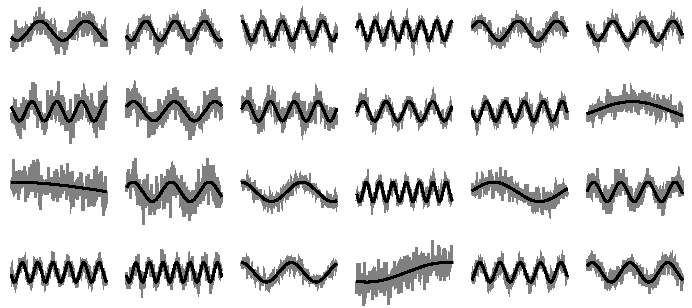
\includegraphics[width=0.8\textwidth]{figures/placeholder.pdf}

\vfill

% ---------------- Footer ----------------

\noindent\rule{\textwidth}{0.8pt}
\vspace{-0.65cm}
\normalsize

\begin{center}
	\begin{minipage}[t]{2.1cm}
	\vspace{0pt}
		
\includegraphics[width=2.02cm]{figures/Logo_AudioLabs.pdf}
	\end{minipage}
	\hfill
	%
	\begin{minipage}[t]{6.88cm}
	\vspace{0pt}
	\centering
	{\fontsize{9.pt}{11pt}\selectfont International Audio Laboratories Erlangen}\\[3pt]
	{\fontsize{7.3pt}{9.5pt}\selectfont\textit{A joint institution of the \\
	Friedrich-Alexander-Universität Erlangen-Nürnberg (FAU) and \\
	the Fraunhofer Institute for Integrated Circuits IIS.\\}}
	\end{minipage}
	%
	\hfill
	\begin{minipage}[t]{2.67cm}
	\vspace{0pt}
		
\includegraphics[width=2.59cm]{figures/Logo_IIS.pdf}
	\end{minipage}
\end{center}

\end{titlepage}

\pagestyle{empty}
\newpage

% ---------------- Preface ----------------
% \cleardoublepage
% \pagenumbering{roman}
% \setcounter{page}{1}
% \pagestyle{fancy}
% \markright{Preface}
% \thispagestyle{sectionfirst}
% \section*{Preface}

{\fontsize{8.5}{12}\selectfont

This book, titled \emph{Preparation Course for Python} (PCP), is about learning Python with a clear destination in mind: the Fourier transform. It introduces the programming tools needed for scientific computing and applies them to a connected sequence of mathematical and signal-processing topics. Step by step, the reader moves from Python and NumPy basics through functions and visualization to complex numbers, exponential functions, signals, sampling, the discrete Fourier transform~(DFT), and finally the fast Fourier transform~(FFT).

This progression provides the guiding thread of the course. Fourier analysis is one of the central tools in science and engineering: it reveals the frequencies contained in a signal and supports numerous methods in signal processing, communications, and data analysis. Understanding the DFT and FFT requires several ideas to come together. Complex numbers provide the natural representation, the exponential function describes oscillations, sampling connects continuous and digital signals, and Python turns these concepts into executable algorithms. The FFT may appear rather mysterious when encountered for the first time. Our aim is to make it feel like the natural conclusion of the journey.

PCP is intended for students in engineering, computer science, and related fields who often bring complementary backgrounds. Some readers may know the mathematics but hesitate when faced with an empty code cell. Others may write Python confidently but feel less at home among complex exponentials and Fourier coefficients. PCP brings these perspectives together through concise explanations, executable examples, visualizations, sound examples, and exercises. No advanced programming knowledge is required; some basic experience with programming or signal processing is helpful, but curiosity and a willingness to experiment are more important.

The material grew out of our teaching at the International Audio Laboratories Erlangen, a joint institution of the Friedrich-Alexander-Universität Erlangen-Nürnberg~(FAU) and the Fraunhofer Institute for Integrated Circuits IIS. In particular, we use PCP as the basis for programming and laboratory courses for students in international Master's programs in computer science, artificial intelligence, data science, and electrical engineering. The follow-on course, the \emph{Preparation Course for PyTorch}~(PCPT)\footnote{\url{https://audiolabs-erlangen.de/PCPT}}, builds on PCP to introduce PyTorch, neural networks, and modern machine learning from a signal-processing perspective. PCP also prepares students for the \emph{Fundamentals of Music Processing}~(FMP)\footnote{\url{https://audiolabs-erlangen.de/FMP}} course, which uses Python to teach central methods for analyzing and processing music signals.

The book is organized into ten units, each corresponding to an executable Jupyter notebook. The opening units introduce the programming environment, Python, NumPy, control structures, functions, and Matplotlib. 

The later units develop the mathematical and signal-processing foundations needed for the DFT and FFT, while the final unit explains how reusable Python code can be organized into modules and packages. Readers may work through the book from beginning to end or return to individual units as a reference. For a first encounter, however, we recommend following the units in sequence, since later concepts and examples build deliberately on earlier ones.

A typical unit begins with an overview and explicit learning objectives. Explanations alternate with executable code so that mathematical statements can be tested immediately and programming ideas can be interpreted in context. Background boxes provide mathematical recaps, historical perspectives, applications, and occasional excursions. Notes emphasize practical conventions and common pitfalls. Exercises conclude each unit and invite the reader to combine the newly introduced ideas. Sample solutions are available through the accompanying \texttt{libpcp} package.

The Jupyter notebooks\footnote{\url{https://audiolabs-erlangen.de/PCP}} form an integral part of the book. They combine text, equations, executable code, figures, exercises, and audio examples in a single interactive document. The complete collection is open source and can be downloaded from GitHub or used through browser-based notebook services. All examples are designed to run on an ordinary notebook computer using freely available software. We encourage readers to modify parameters, create additional examples, and treat the notebooks not as fixed demonstrations but as starting points for their own experiments.

The PCP notebooks were first developed together with Sebastian Rosenzweig, whose ideas and contributions played a central role in shaping the course. We gratefully acknowledge the work and feedback of Vlora Arifi-Müller, Michael Krause, Heinrich Löllmann, Peter Meier, and Frank Zalkow, as well as the many students whose questions, difficulties, and suggestions helped us improve the material. The project also benefited from our collaboration with colleagues in the music-processing, signal-processing, and machine-learning communities.

Our broader goal is to promote a style of learning in which programming and mathematics reinforce one another. A formula should not remain an isolated symbolic statement when it can be turned into an experiment, and a piece of code should not remain a collection of instructions when its mathematical structure can be understood. We hope that readers finish the course not only with greater confidence in Python but also with a clearer sense of how computational thinking can make abstract ideas concrete.

By the end of the book, the FFT should no longer appear as a mysterious black box. It should emerge as a carefully organized computation built from familiar elements: arrays, functions, complex numbers, roots of unity, sampled signals, and the DFT. More importantly, readers should be prepared to approach new computational methods in the same spirit, connecting mathematical structure, executable code, and critical experimentation.

\vspace{2em}

\noindent
Erlangen, October 2026\\
Meinard Müller and Sebastian Strahl

}


% ---------------- Table of Contents ----------------
\cleardoublepage
\renewcommand{\contentsname}{Contents \\}
\markright{}
\tableofcontents
\thispagestyle{fancy}
\pagestyle{empty}
\newpage

% ---------------- Include PDFs ----------------
\cleardoublepage
\pagenumbering{arabic}
\setcounter{page}{1}
\pdfsection{Introduction}{intro}{../../PCP.pdf}
\pdfsection{Unit 1: Get Started}{getstarted}{../../PCP_01_getstarted.pdf}
\pdfsection{Unit 2: Python Basics}{classes}{../../PCP_02_python.pdf}
\pdfsection{Unit 3: NumPy Basics}{tensor}{../../PCP_03_numpy.pdf}
\pdfsection{Unit 4: Control Structures and Functions}{grad}{../../PCP_04_control.pdf}
\pdfsection{Unit 5: Visualization Using Matplotlib}{nn}{../../PCP_05_vis.pdf}
\pdfsection{Unit 6: Complex Numbers}{convolution}{../../PCP_06_complex.pdf}
\pdfsection{Unit 7: Exponential Function}{classification}{../../PCP_07_exp.pdf}
\pdfsection{Unit 8: Signals and Sampling}{training}{../../PCP_08_signal.pdf}
\pdfsection{Unit 9: Discrete Fourier Transform (DFT)}{recursion}{../../PCP_09_dft.pdf}
\pdfsection{Unit 10: Python Modules and Packages}{essential}{../../PCP_10_module.pdf}

\end{document}
